\chapter[Analyse fonctionnelle]{Analyse fonctionnelle}

\textit{Le présent chapitre a pour objectif de présenter la structuration de l'application. La modélisation du problème va influencer l'organisation des données du programme. De plus, différentes fonctionnalités doivent être implémentées pour agir sur ces données.}

\section{Contraintes de modélisation du projet}

Les principales contraintes de développement de l’interface sont liées à la modélisation du problème. Deux choix sont possibles : une modélisation multi-classe, et une modélisation multi-label. Dans le premier cas, les objets classés sont répartis sur plusieurs classes, tout en sachant qu’un objet ne peut appartenir qu'à une seule classe. Dans le cas de la modélisation multi-label, un objet peut appartenir à plusieurs labels, chacun proposant un choix binaire (appartenance/non-appartenance).\newline

\begin{figure}[!h]
	\begin{center}
		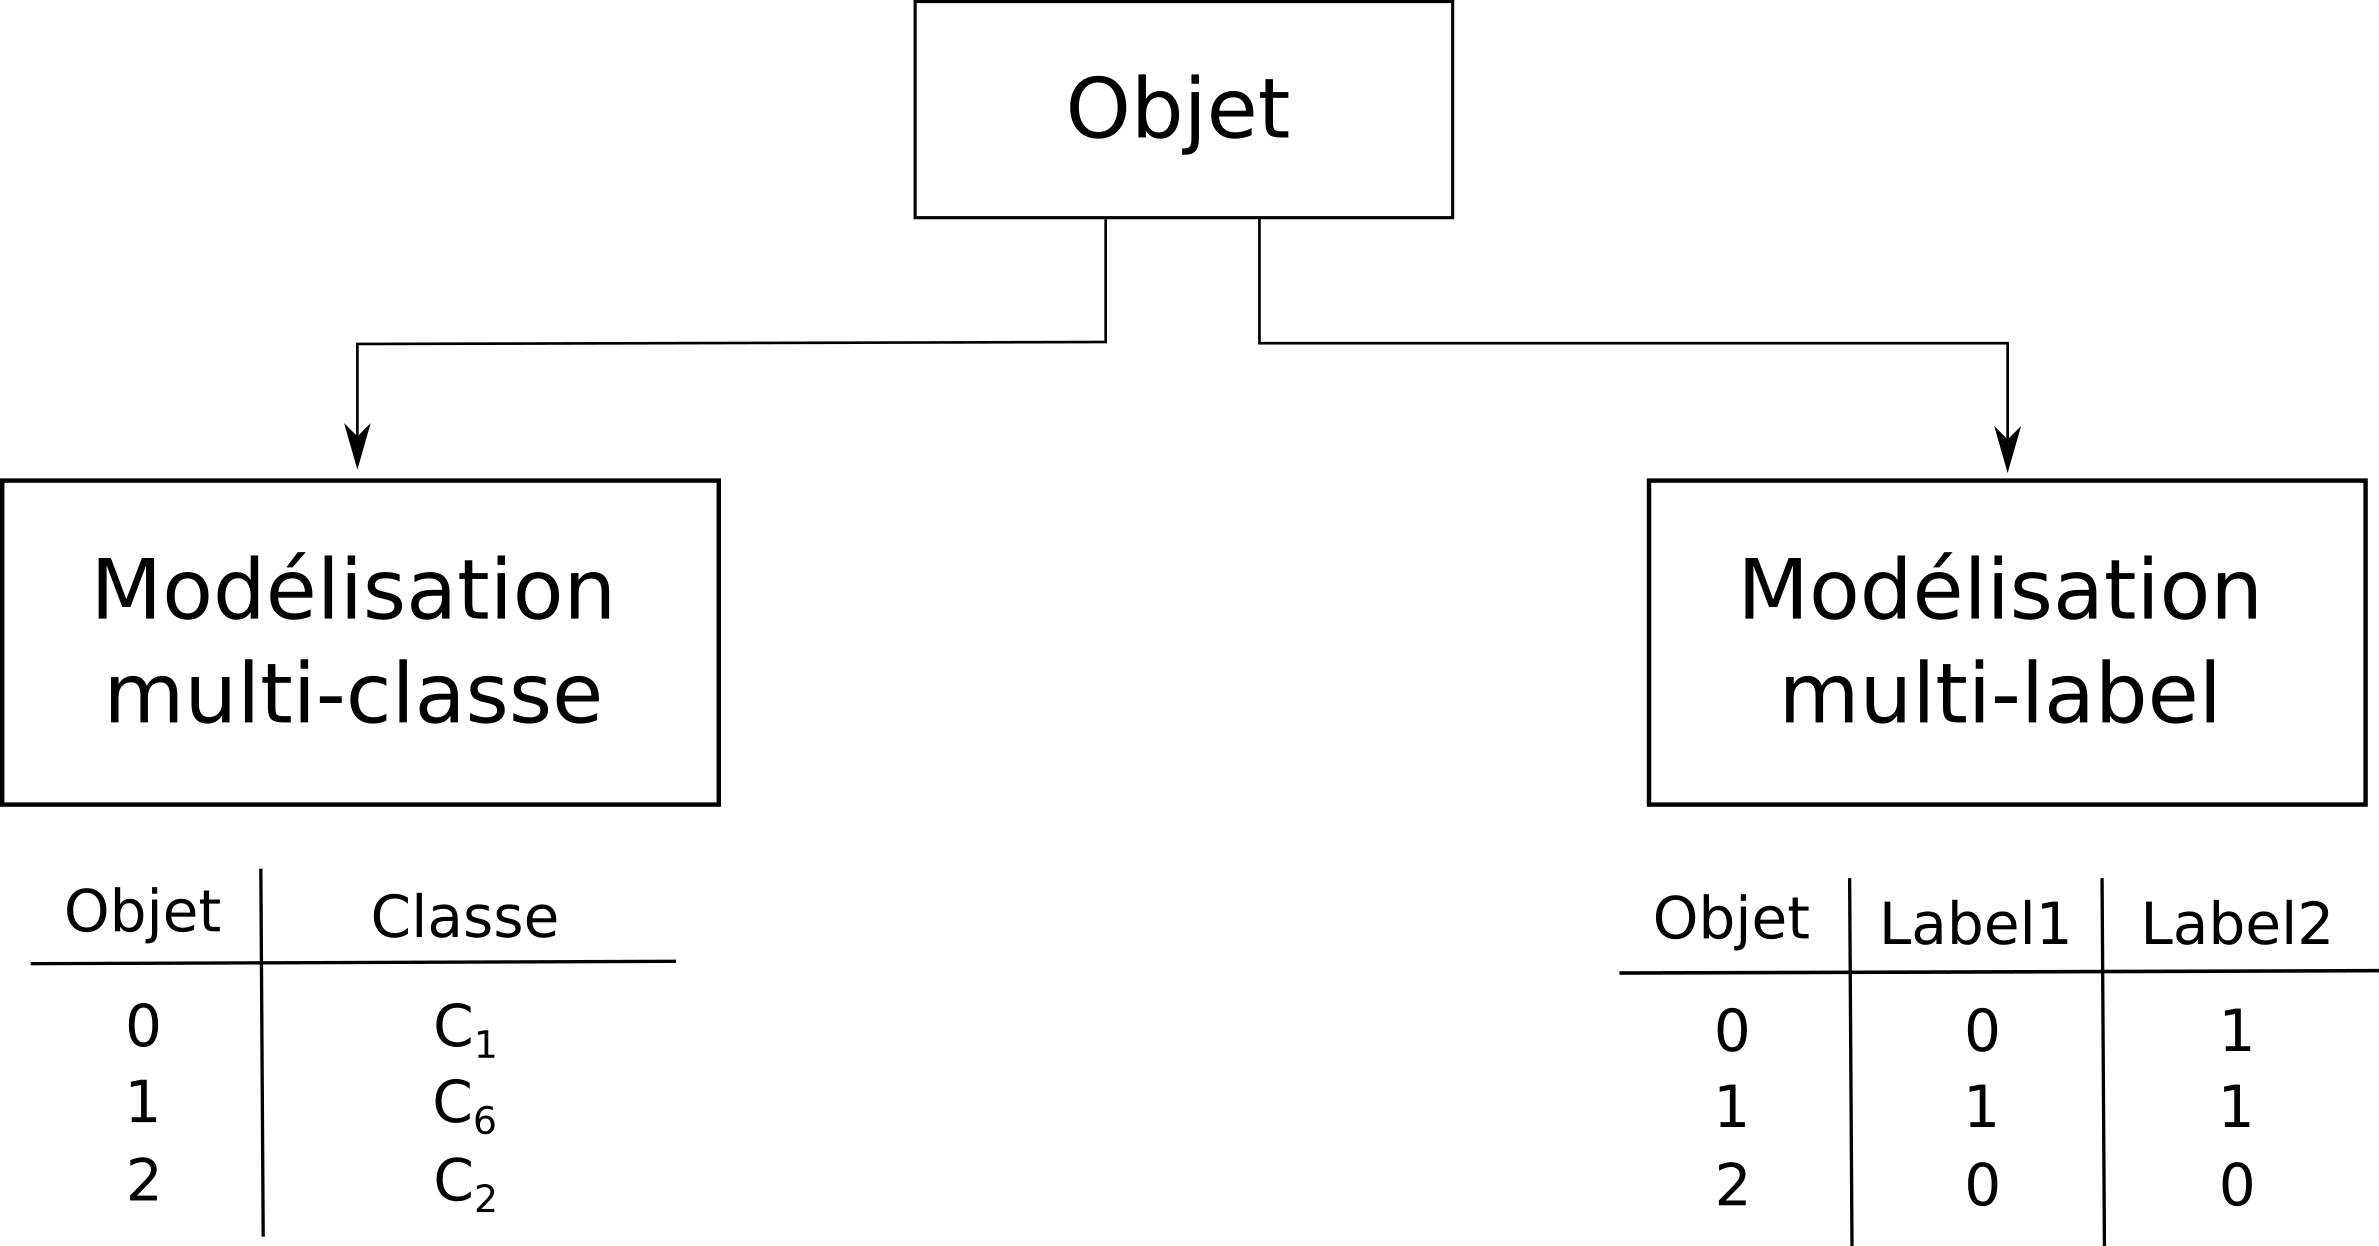
\includegraphics[scale=0.5]{modelisation.png}  \\
		\caption[Modélisation du problème]{Modélisation du problème}
		\label{fig:modelisation}
	\end{center}
\end{figure}

Le choix de la modélisation du problème a un impact sur le formalisme des données en entrée et en sortie du programme. Le choix de l’interface à montrer sera aussi déterminé par la modélisation. Ainsi, dans le cas multi-classe, un objet classifié ne sera lié qu’à une seule erreur. Cela implique que l'utilisateur ne peut choisir qu'une seule classe d'erreur. \newline

Pour l'implémentation de l’interface, le modèle multi-classe a été privilégié pour premier objectif. Une fois cet objectif atteint, on pourra évoluer vers une modélisation multi-label. L’interface programmée doit donc être flexible pour prendre en compte les différents formalismes. \newline

Le choix de modélisation du problème impacte le formalisme des données nécessaires. Ainsi, après avoir décrit les contraintes liées au projet, on peut analyser les données en entrée et en sortie du programme.\newline

\section{Organisation des données}

\subsection{Données en entrée}

La première étape d'analyse concerne les données en entrée, dans le cas d'une modélisation multi-classe. On considère 4 jeux de données en entrée :
\begin{itemize}[label=$\rightarrow$]
	\item Un fichier CSV (Comma-Separated Values) qui regroupe les classes d’erreurs possibles et leur description.
	\item Un fichier CSV qui regroupe les résultats de la phase de classification. Pour chaque entité, on retrouve son identifiant, sa classe et sa probabilité d’appartenance à cette classe.
	\item Un dossier qui regroupe les emprises des entités au format shapefile (SHP). L’identifiant de l’entité se retrouve dans le nom du fichier d'emprise (\emph{ex : « 2516.SHP » pour l’entité 2516}).
	\item Une orthoimage au format TIFF de la zone analysée, spatialement superposable aux fichiers d’emprise.\newline
\end{itemize}

L’ensemble de ces données doit être fourni par l’utilisateur avant l’exécution du programme. Pour cela, une fenêtre de chargement des fichiers doit être implémentée. \newline

\begin{figure}[H]
	\begin{center}
		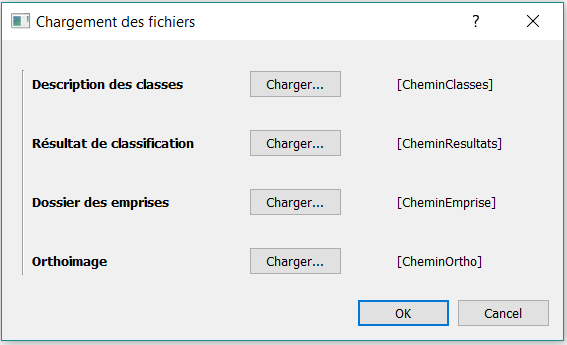
\includegraphics[scale=0.70]{Interf_chargement}  \\
		\caption[Maquette de l'interface de chargement des fichiers]{Maquette de l'interface de chargement des fichiers}
		\label{fig:interfCharg}
	\end{center}
\end{figure}

\subsection{Données en sortie}

\noindent En sortie de l'interface, un seul fichier est retourné :
\begin{itemize}[label=$\rightarrow$]
	\item Un fichier CSV qui regroupe les résultats de l'interaction avec l'utilisateur. On retrouve un formalisme identique au fichier des résultats de classification donné en entrée (identifiant, classe, probabilité). Deux méthodes sont envisageables : une première hypothèse consiste à sortir un tableau avec l'ensemble des entités testées (qu'elles soient modifiées ou non), et une seconde à ne restituer que les entités qui ont été modifiées.\newline
\end{itemize}

\subsection{Structuration des données}

\noindent\textbf{Lecture des fichiers CSV}\\

Les données au format CSV (Comma-Separated Values) concernent les fichiers qui regroupent les classes et les résultats de classification. Ce format permet d’enregistrer des données tabulaires sous forme de valeurs séparées par des virgules. \newline

\noindent Dans le programme, les fichiers seront traduits de manières différentes :

\begin{itemize}[label=$\rightarrow$]
	\item Pour le fichier qui regroupe les classes, les données seront enregistrées dans une variable de type dictionnaire. Ces données ne vont pas évoluer au cours du processus, ce qui justifie ce formalisme. Il sera ainsi possible d'accéder aux descriptions des classes via les valeurs des clés du dictionnaire.
	\item Pour le fichier qui contient les résultats de classification, les données seront enregistrées comme une liste de tuples. En effet, ce type de variable est facilement manipulable avec Python. Cette liste servira pour filtrer les bâtiments à afficher.\\
\end{itemize}

\noindent\textbf{Lecture des données graphiques}\\

Le format SHP est un format de fichier utilisé pour les systèmes d'informations géographiques (SIG). Il permet de stocker des entités SIG vectorielles. Dans notre cas, on utilise ce format pour les emprises des bâtiments orthoprojetés. Après avoir sélectionné les entités à présenter, on utilisera ces données de géométrie pour créer une classe "Bâtiment".\\

La lecture de l'orthophoto au format TIFF (Tagged Image File Format) permet d'obtenir des informations quant à la géométrie de l'image (coordonnée du point origine, taille du pixel,...). Elle ne sera lu que lors de l'affichage pour limiter l'enregistrement de données.\\

Pour le projet, on considère que les emprises et l'orthophoto sont représentées dans le même repère. Il ne sera donc pas nécessaire de gérer les projections.\\

\section{Analyse fonctionnelle}

Après avoir analysé les données nécessaires au programme et leur formalisme, on peut définir les différentes fonctionnalités du projet et leur organisation.\newline

\subsection{Principales fonctionnalités du programme}

L'interface doit permettre de visualiser et contrôler les résultats d'une classification.

\begin{figure}[h]
	\begin{center}
		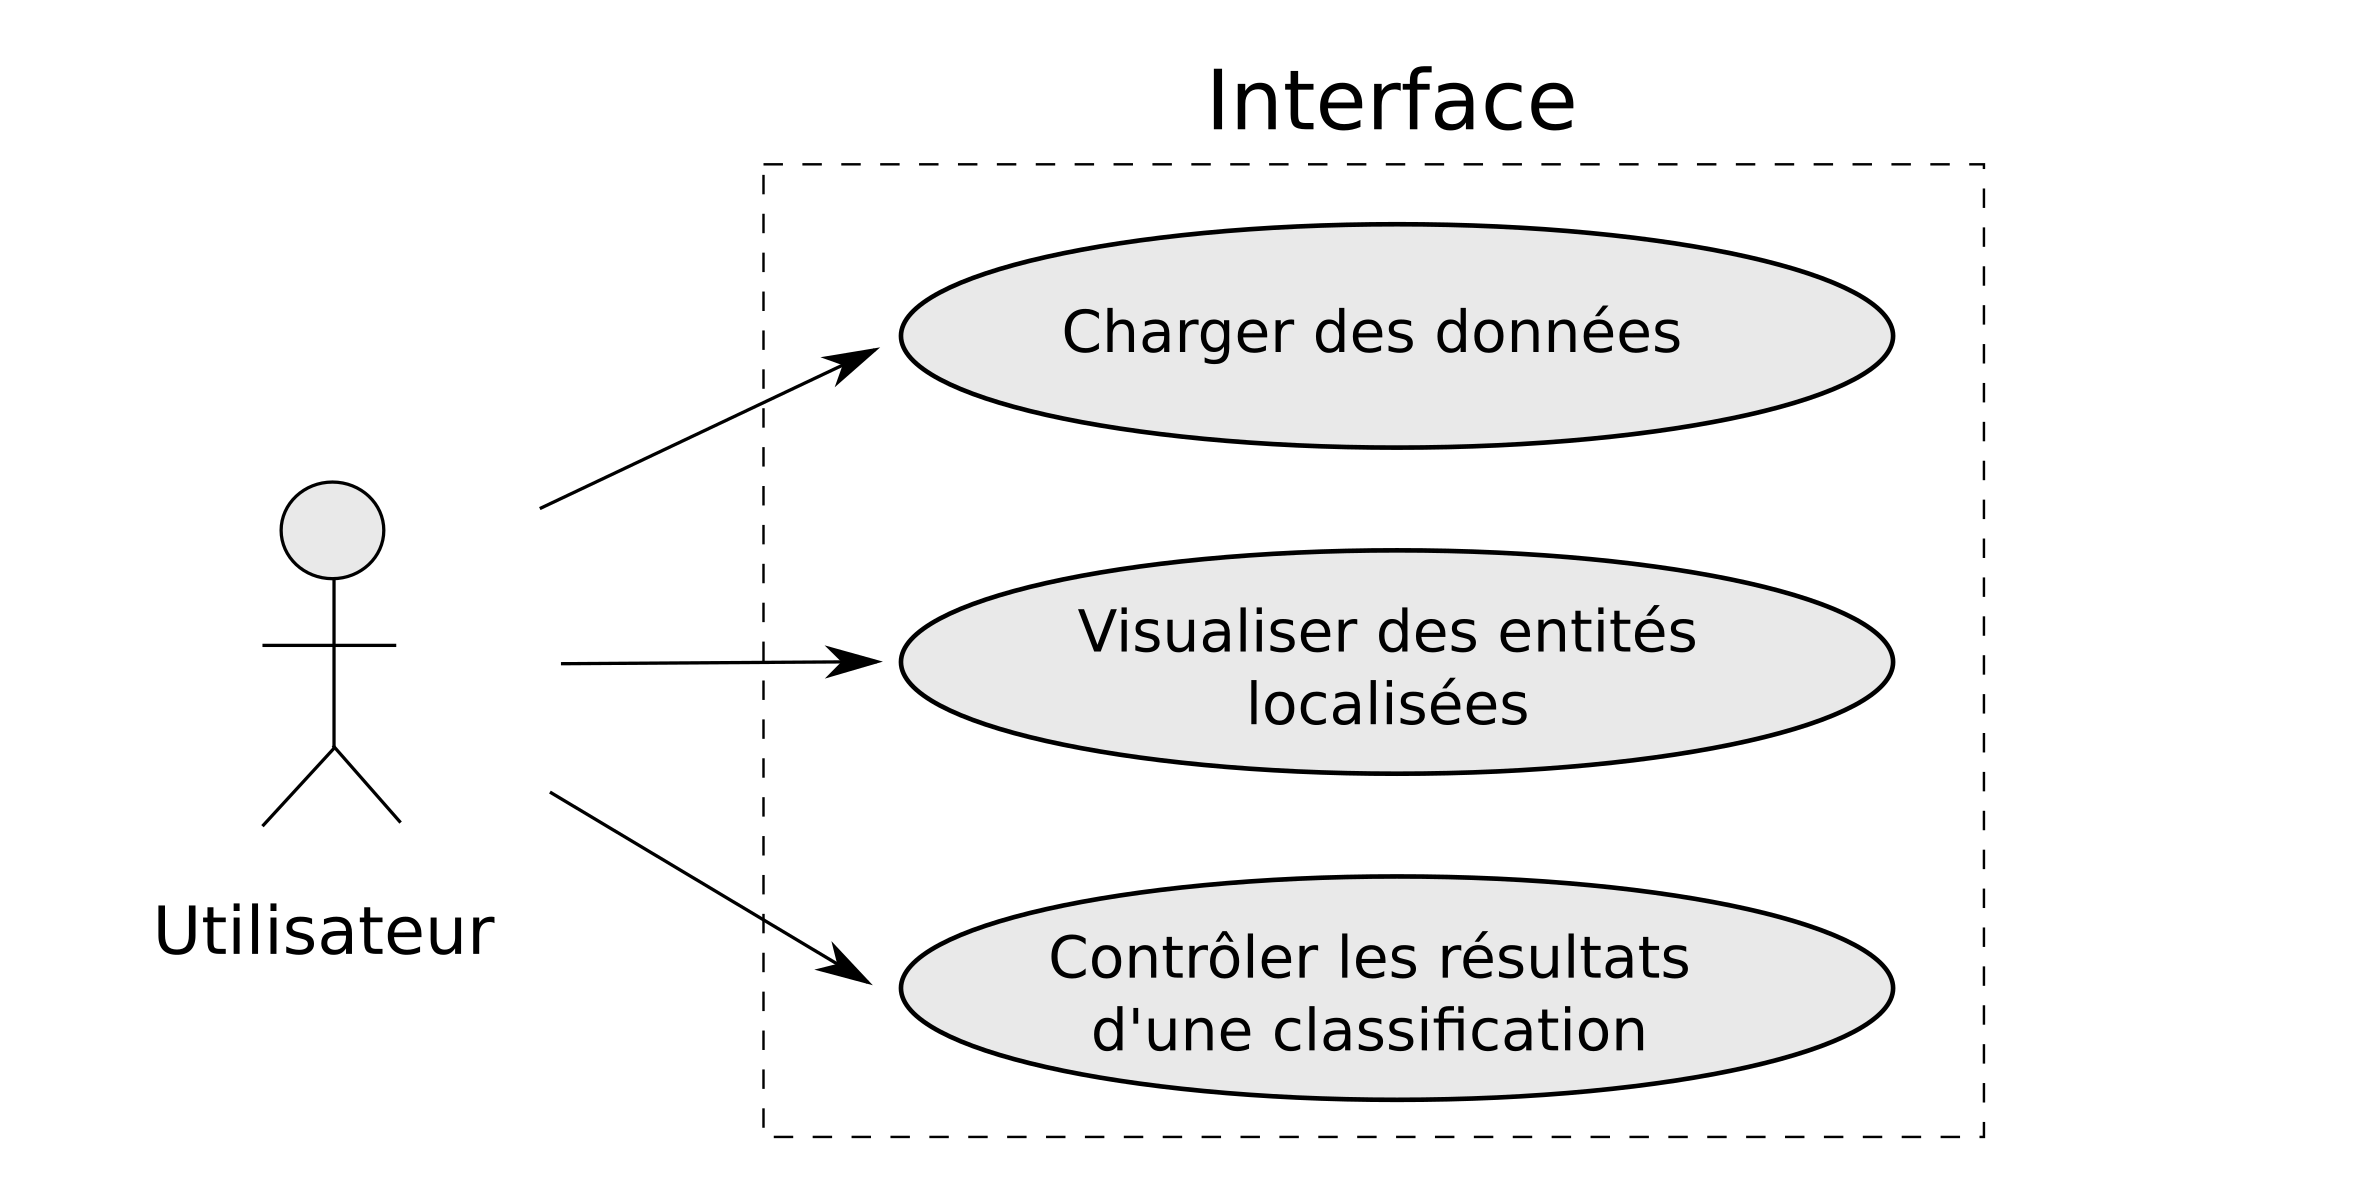
\includegraphics[scale=0.6]{diagramme_cas_utilisation.png}  \\
		\caption[Cas d'utilisation]{Cas d'utilisation}
		\label{fig:utilisation}
	\end{center}
\end{figure}


\subsection{Organisation générale des fonctions}

Le diagramme fonctionnel ci-dessous permet de représenter sous forme de blocs fonctionnels l'ensemble du système étudié. Ces fonctionnalités doivent permettre de répondre aux cas d'utilisation de l'interface.

\begin{figure}[H]
	\begin{center}
		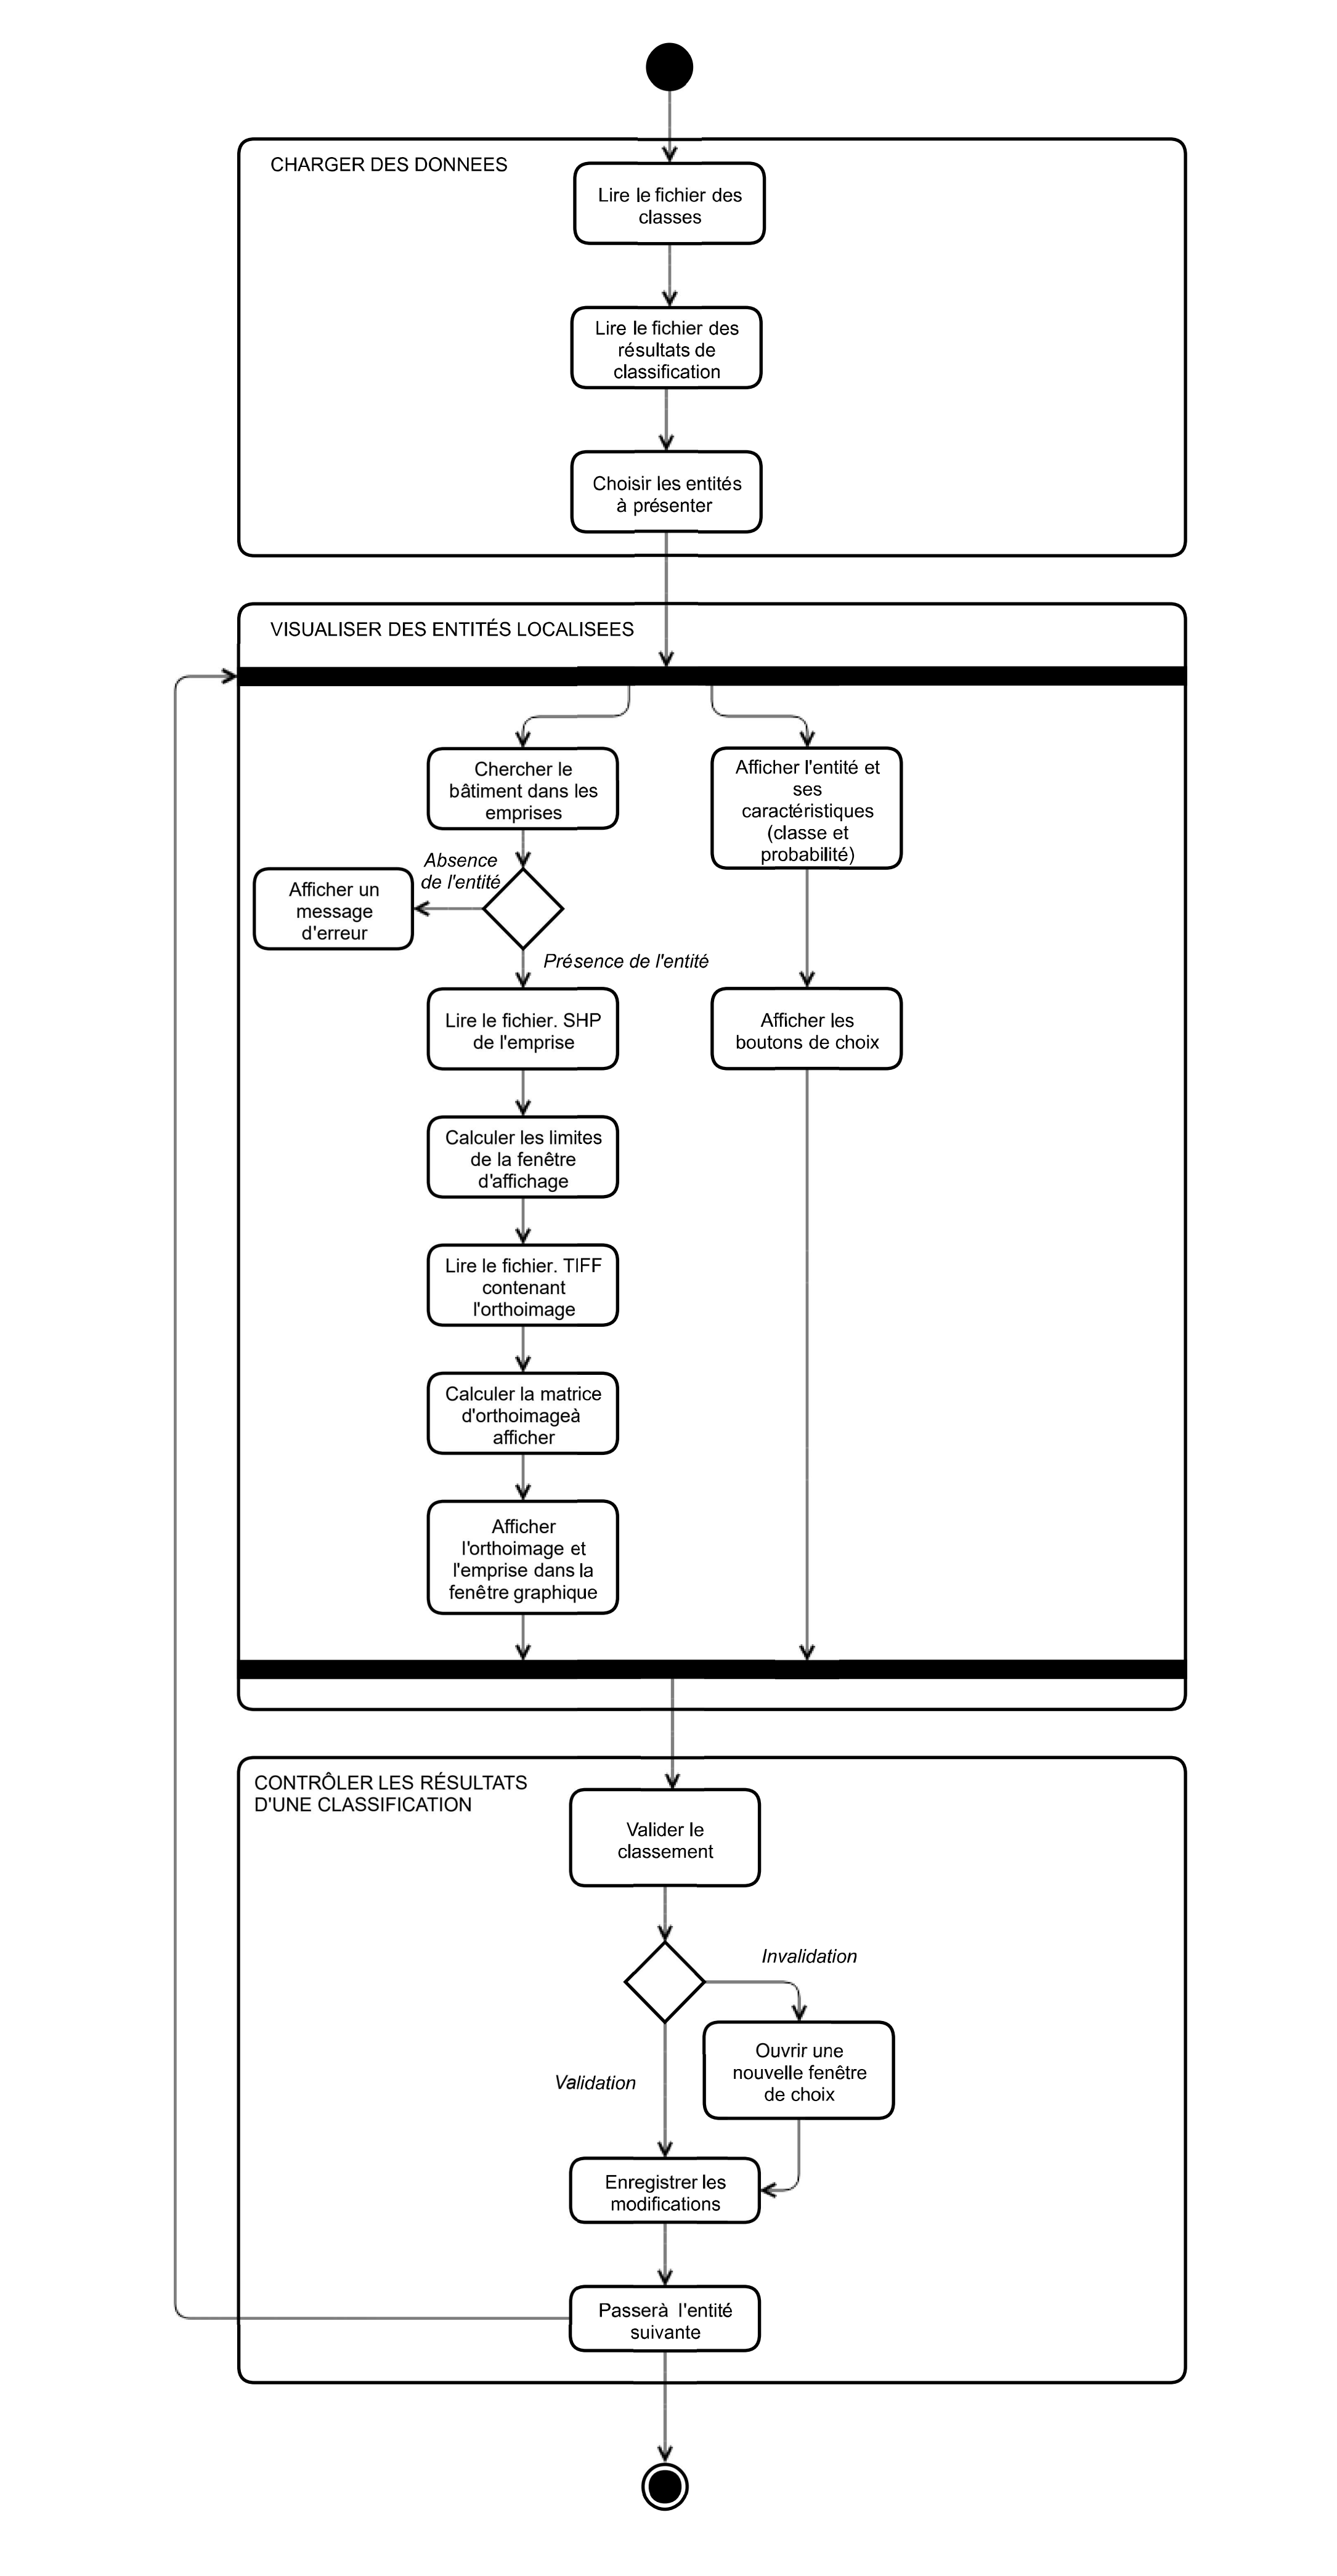
\includegraphics[scale=0.80]{Analyse_fonctionnelle.png}  \\
		\caption[Diagramme fonctionnel]{Diagramme fonctionnel}
		\label{fig:fonction}
	\end{center}
\end{figure}

\subsection{Détail des fonctions}

Après avoir schématisé l'ensemble des fonctionnalités à implémenter, on détaille le fonctionnement des principales fonctions.\\

\noindent\textbf{Fonction de sélection des entités}\\

Cette fonction doit permettre à l’utilisateur de choisir la stratégie d’affichage des entités résultant de la classification. En effet, l’objectif n’est pas que l’utilisateur contrôle l’ensemble des données, mais seulement celles qui influent le plus sur la classification.\newline

\noindent Plusieurs stratégies d’affichages peuvent être envisagées :
\begin{enumerate}
	\item L’affichage de toutes les entités
	\item L'affichage d'entités aléatoirement choisies
	\item L’affichage des entités dont la probabilité d’appartenance est la plus faible
	\item L’affichage des entités ayant des conflits de classification (cas des erreurs ayant des probabilités très proches)
\end{enumerate}

Dans les deux derniers cas, des entités aléatoires devront également être affichées. En effet, si l’on souhaite améliorer le processus global de classification, l’utilisateur doit agir sur toutes les classes.\\ 

\noindent Deux types de traitements sont envisageables : 
\begin{enumerate}
	\item Un traitement offline, qui sélectionne les entités à afficher indépendamment de la requalification par l’utilisateur
	\item Un traitement online, qui va sélectionner un échantillon de données qui va être remis à jour selon les résultats du reclassement
\end{enumerate}

Dans un premier temps, on se limitera au filtrage offline afin de faciliter l'implémentation et de se concentrer sur le fonctionnement global de l’interface. De plus, les différentes méthodes de filtrage seront organisées sous forme de classes pour faciliter la transition de l'une à l'autre. \\

\noindent\textbf{Manipulation des fichiers SHP des bâtiments orthoprojetés}\\

Une fois les entités à afficher sélectionnées, on cherche à lire les fichiers SHP correspondant. Ces emprises sont stockées dans un dossier unique, et leur nom correspond à l'identifiant de l'entité. Dans la première implémentation, en cas d’absence de l’emprise dans le dossier, cette fonction devra afficher une fenêtre d’erreur à l’utilisateur.\newline 

Grâce à la lecture des fichiers, on renseigne des objets de type "Bâtiment" avec un identifiant, une géométrie, une classe et une probabilité. \newline

Une dernière étape consistera à calculer, pour chaque emprise, les bornes d’affichage qui lui sont liées. Cela nécessite de déterminer la fenêtre d’affichage ([$x_{min}$,$y_{min}$] et [$x_{max}$,$y_{max}$]) lors de la lecture du fichier. Les marges ($m_x$,$m_y$) définies par l’utilisateur sont ensuite rajoutées aux coordonnées pour obtenir les angles repères de la fenêtre graphique ([$x_h$,$y_h$] et [$x_b$,$y_b$]).\newline

\begin{figure}[H]
	\begin{center}
		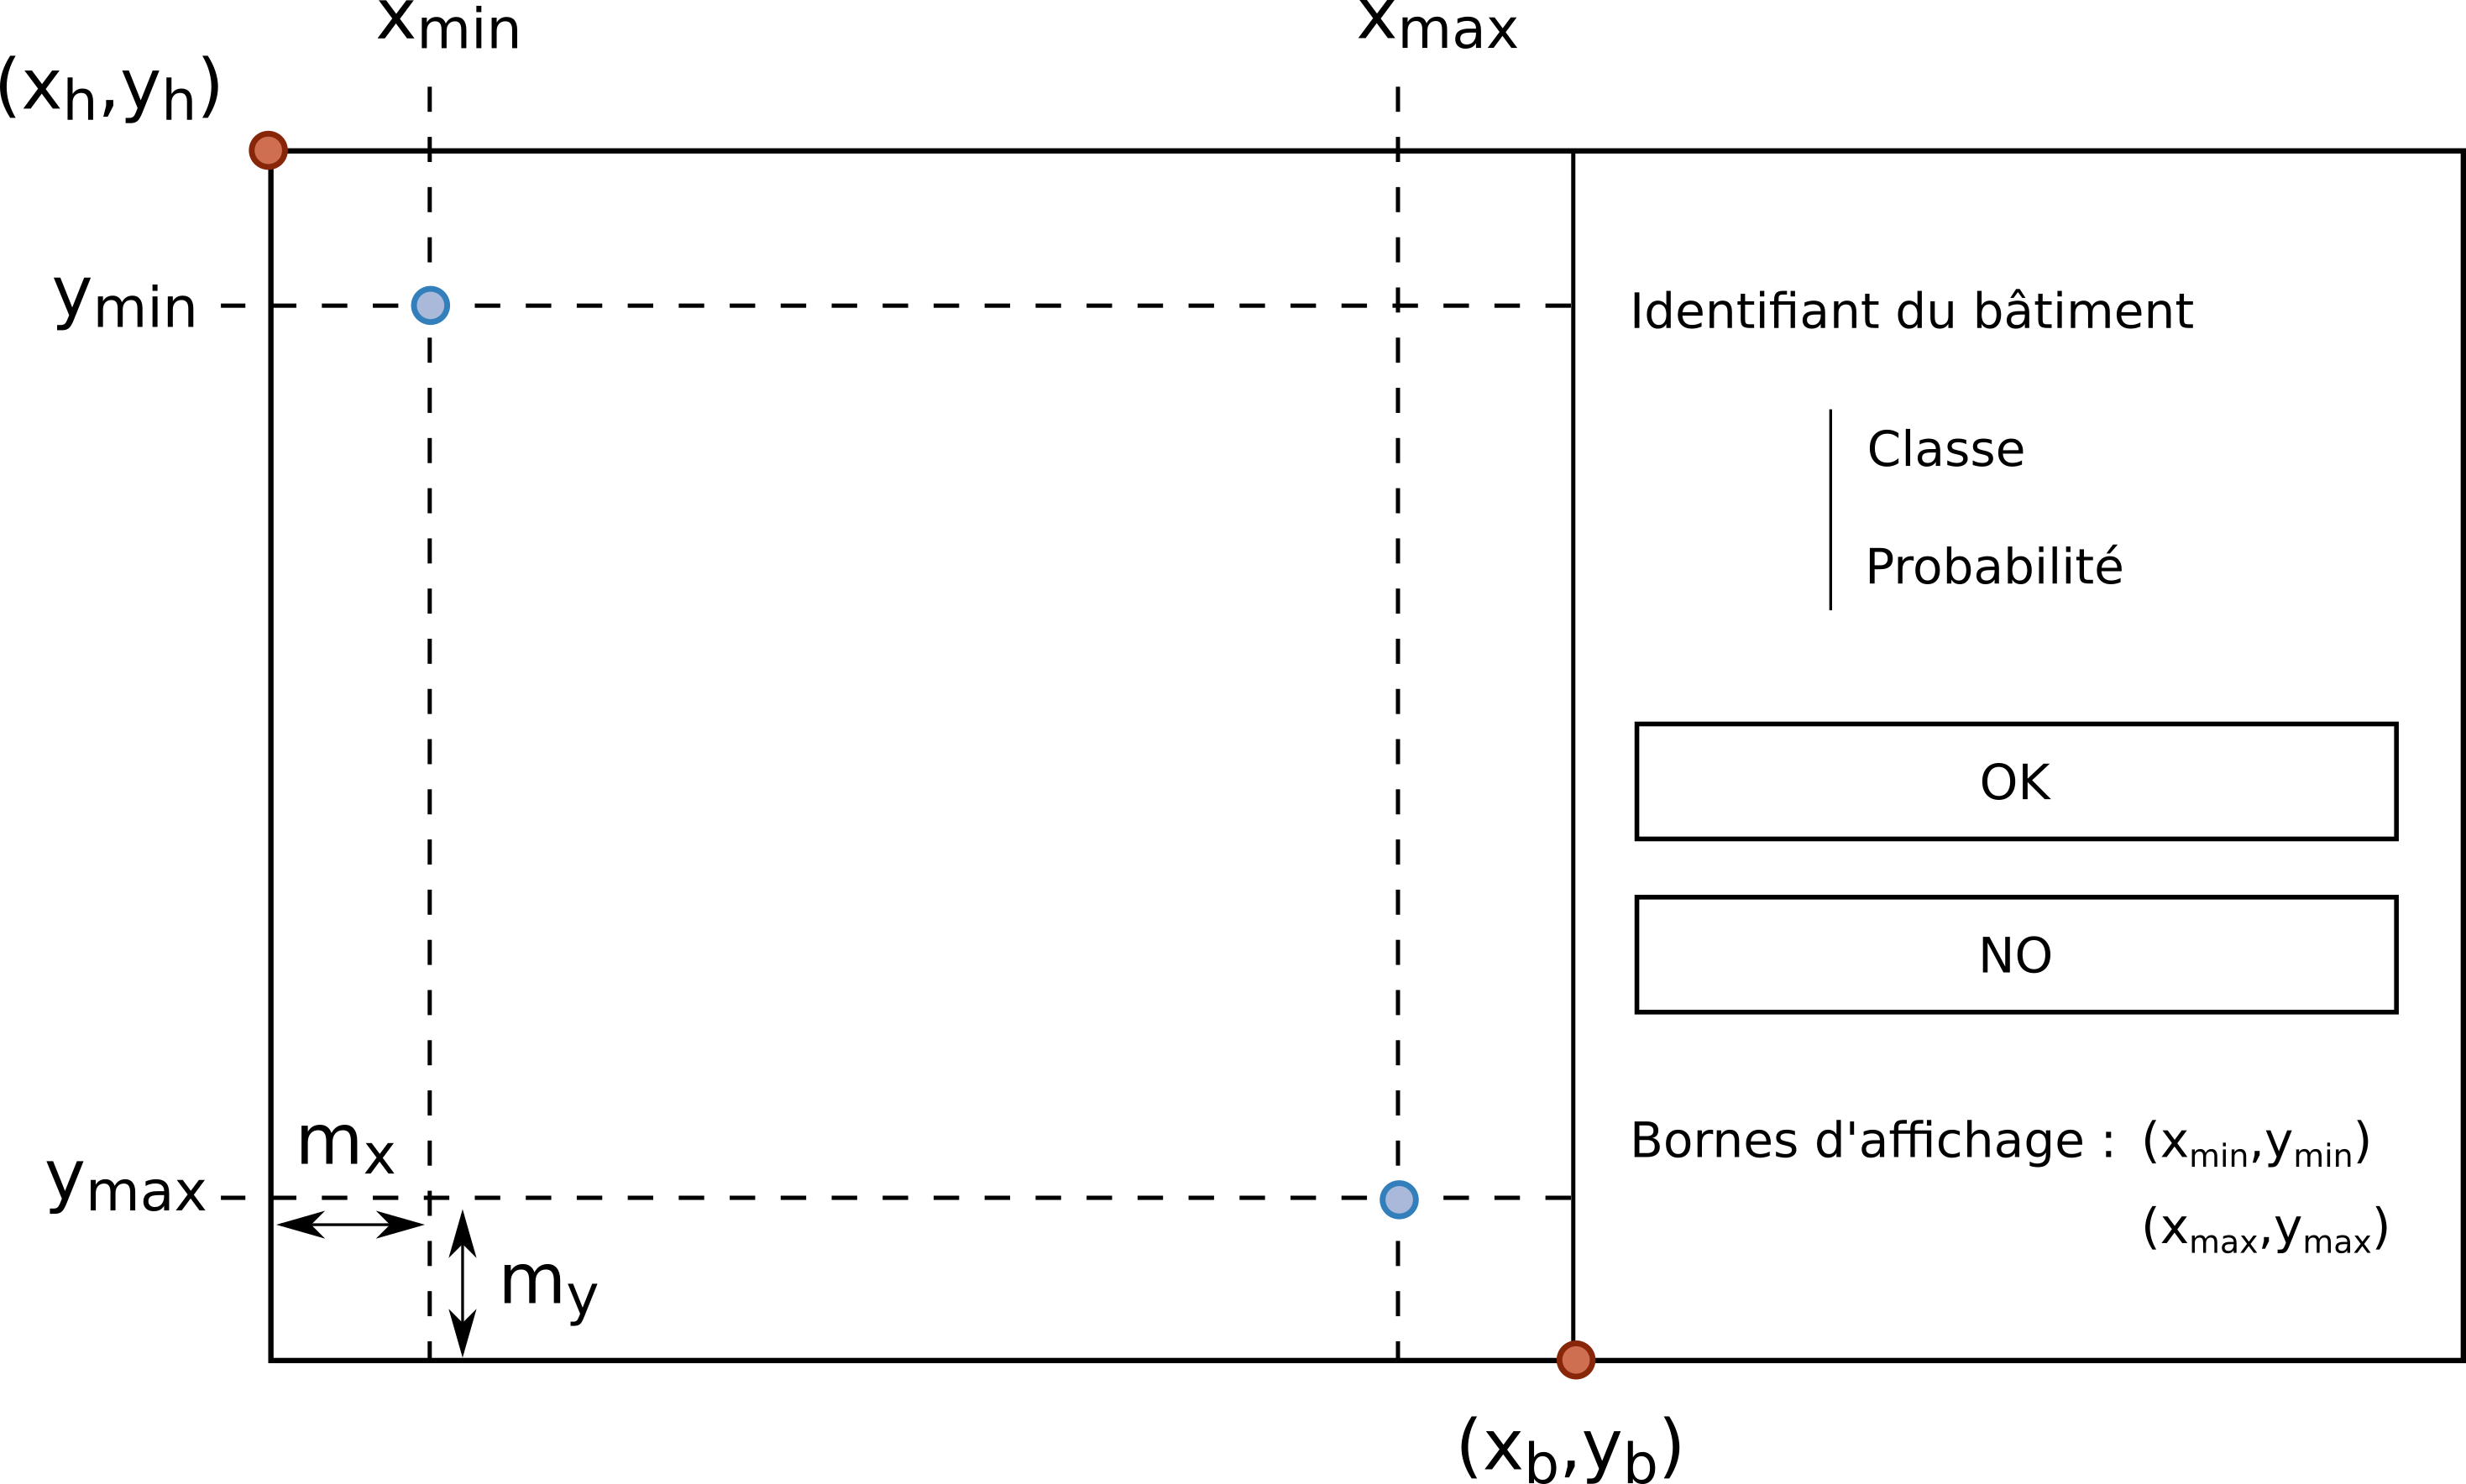
\includegraphics[scale=0.4]{interface_schema.png}  \\
		\caption[Schéma d'organisation de l'interface]{Schéma d'organisation de l'interface}
		\label{fig:interfaceschema}
	\end{center}
\end{figure}

\noindent\textbf{Analyse de l'orthophoto}\\

La lecture du fichier TIFF de l’orthophoto doit nous permettre de trouver son point d’origine ainsi que la taille d’un pixel. Les emprises étant spatialement superposables à l’orthophoto, on utilise les valeurs des bornes d’affichage des emprises pour calculer la matrice d’orthoimage à afficher. Dans la fenêtre graphique, on lui superpose l’emprise du bâtiment.\newline

\noindent\textbf{Phase d'interaction avec l'utilisateur}\\

L’affichage des informations relatives à l’entité permet à l’utilisateur de contrôler les résultats de la classification :
\begin{itemize}[label=$\rightarrow$]
	\item Si l’utilisateur valide le résultat, celui-ci est enregistré et la fenêtre affiche l’entité suivante.
	\item Si l’utilisateur ne valide pas le résultat, une nouvelle fenêtre s’ouvre et propose les autres choix possibles. L’utilisateur ne peut sélectionner qu’une seule proposition, puis valide. Une fois le résultat enregistré, on affiche l’entité suivante.
\end{itemize}

\section{Conception de l'interface}

Après avoir analysé les données et les fonctionnalités de l'interface, on s'intéresse à l'organisation du programme.

\subsection{Méthode Modèle/Vue/Contrôleur}

Pour faciliter l’écriture et la compréhension du code de l’interface, on utilisera la méthode Modèle/Vue/Contrôleur :

\begin{itemize}[label=$\rightarrow$]
	\item Le fichier "Modèle" contiendra les données à afficher en entrée et les résultats en sortie.
	\item Le fichier "Vue" contiendra le code de l’interface graphique.
	\item Le fichier "Contrôleur" contiendra les définitions informatiques des actions effectuées par l’utilisateur dans l’interface (\emph{ex : actions à exécuter lors de la validation de la classification, …}). Ces actions viendront modifier les données contenues dans le modèle, ce qui va entrainer un changement dans la vue.
\end{itemize}

\begin{figure}[H]
	\begin{center}
		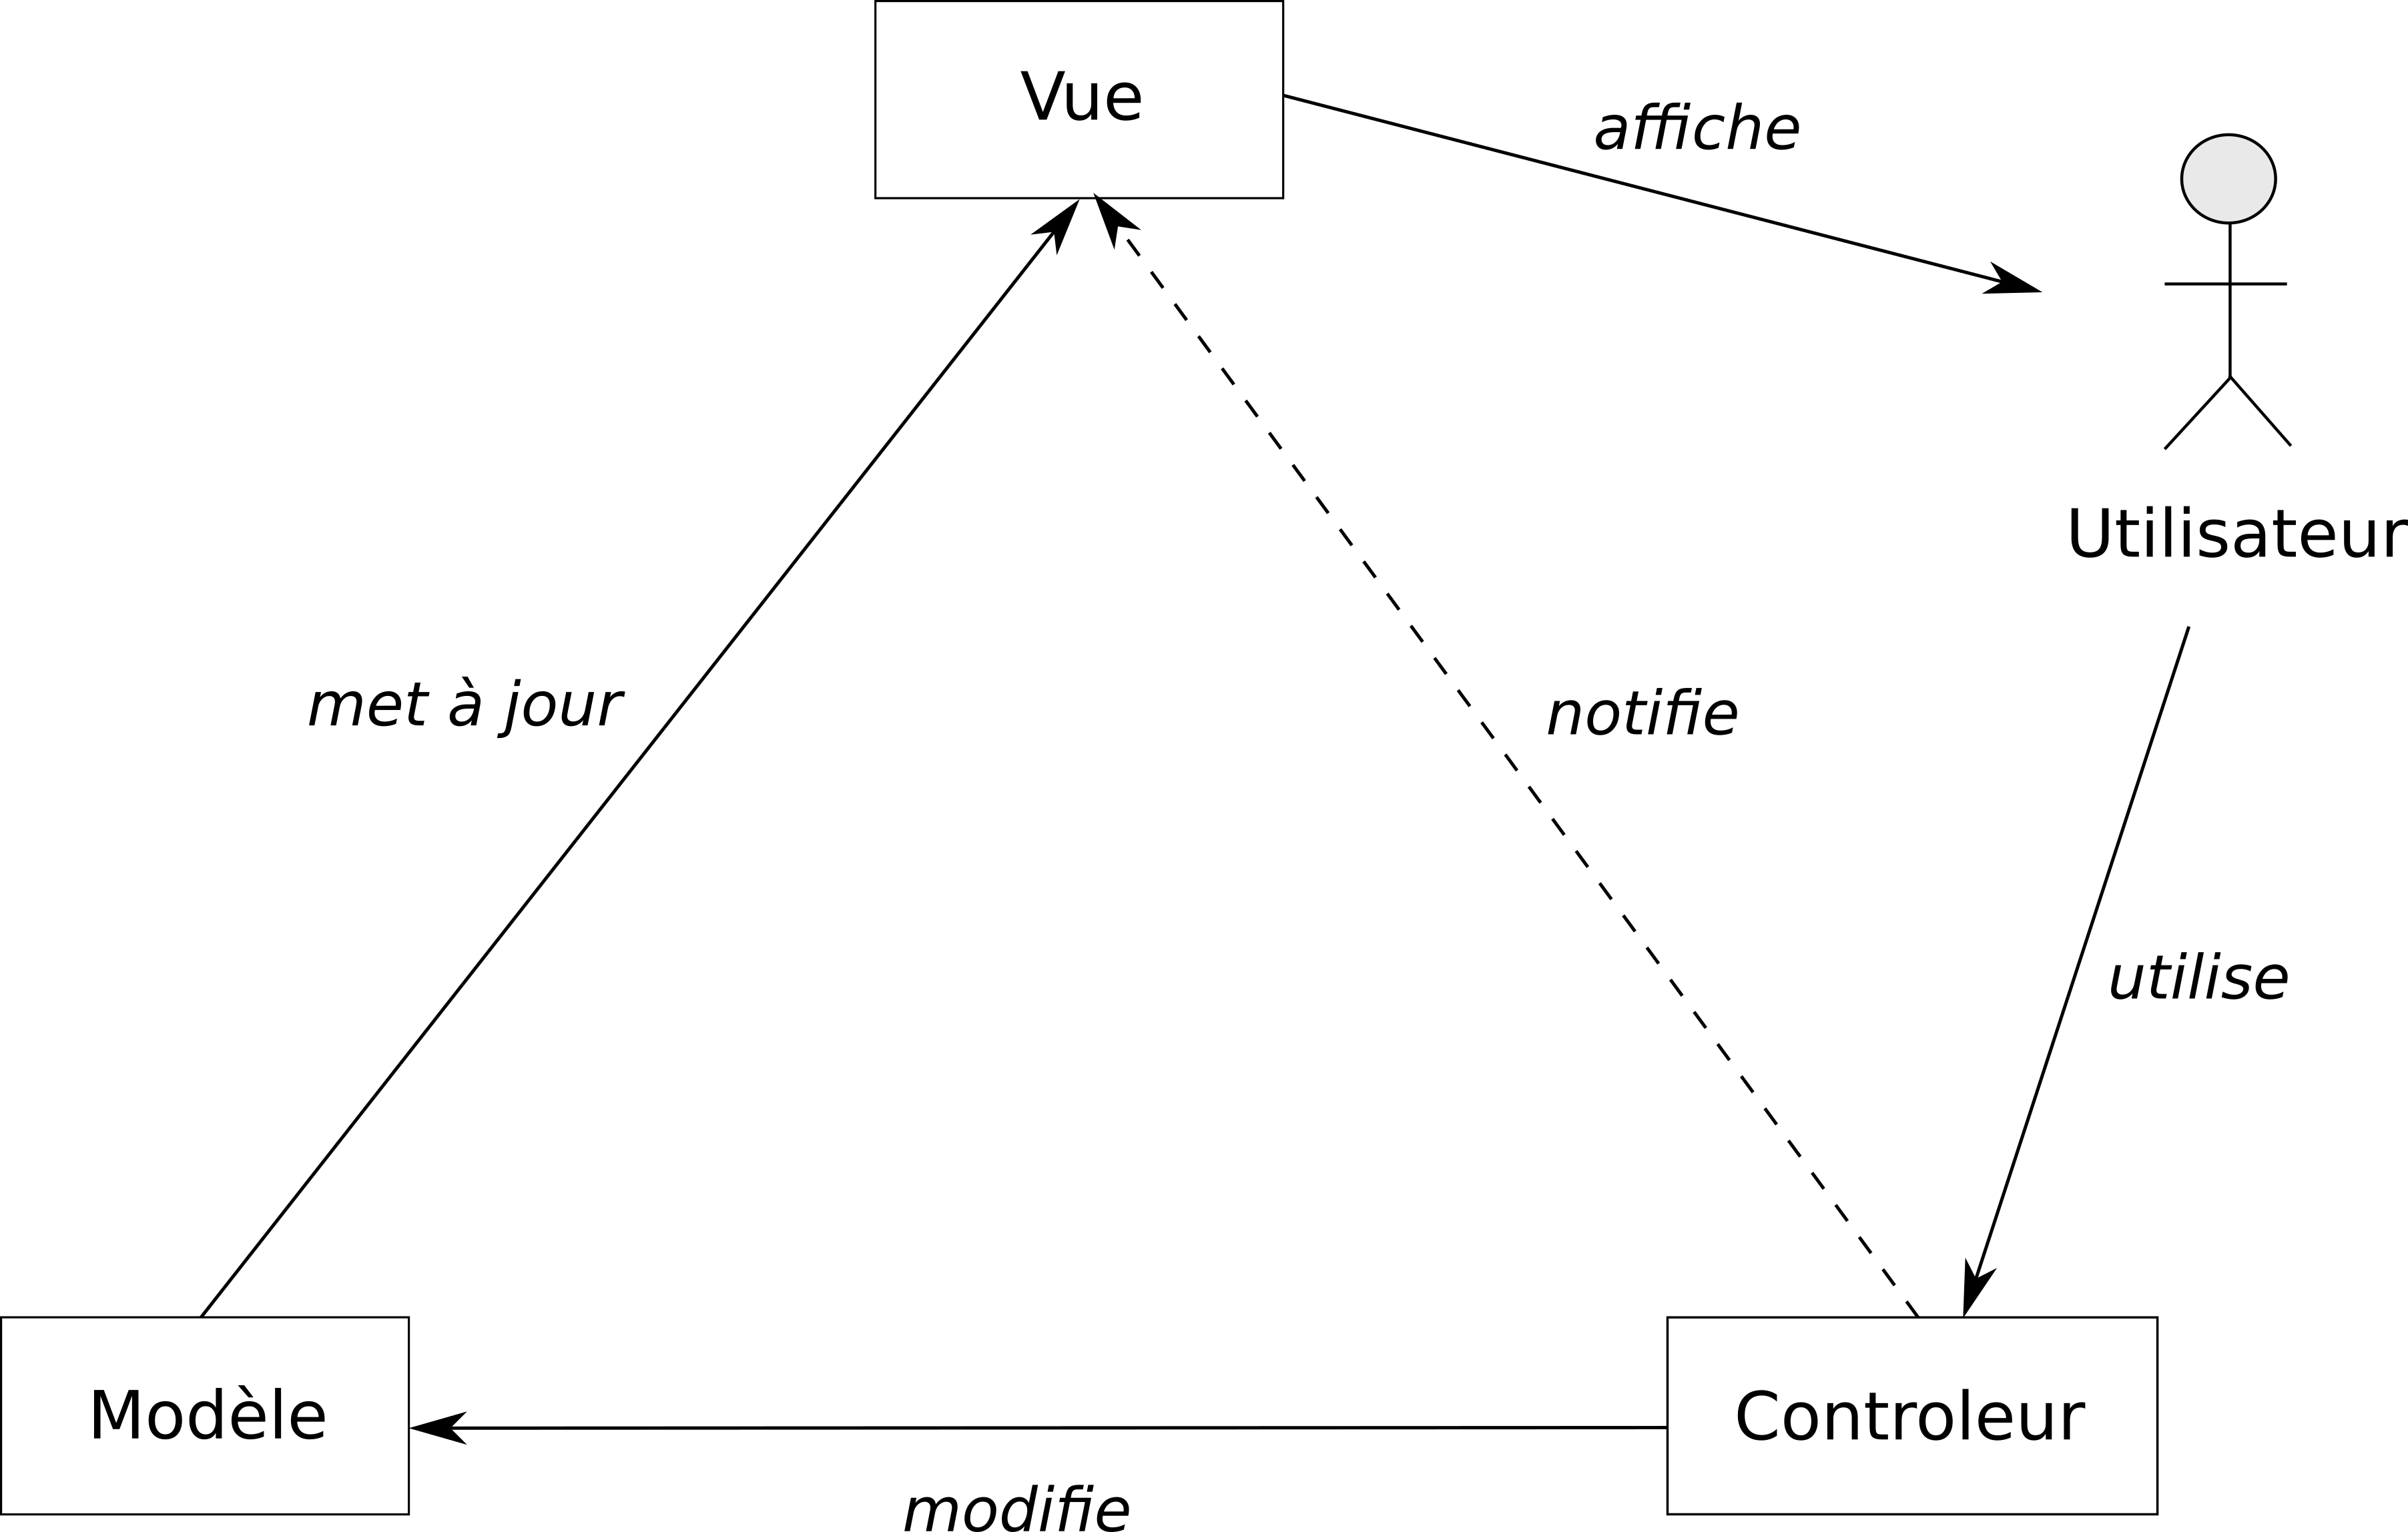
\includegraphics[scale=0.28]{MVC.png}  \\
		\caption[Agencement Modèle/Vue/Contrôleur]{Agencement Modèle/Vue/Contrôleur}
		\label{fig:MVC}
	\end{center}
\end{figure}

\subsection{Diagramme de classe}

Les différents fichiers définis plus haut vont permettre d'agencer le code de manière claire. A l'intérieur de ces trois fichiers, on définira les différentes fonctions mais aussi des classes.\\

La partie "Vue" correspond à l'interface graphique. Comme on le verra par la suite, on s'appuiera sur Qt et QtCreator pour mettre au point cette fenêtre. Ainsi, les classes présentes dans le fichier vue seront gérées par Qt.\\

La partie "Modèle" est celle qui définit les actions réalisables par l'utilisateur. Dans ce fichier, on pense définir deux classes :
\begin{itemize}[label=$\rightarrow$]
	\item Une classe abstraite "Statégie" qui sélectionnera les entités à afficher en appliquant un filtre sur les données en entrée. Les types stratégies seront définies dans des classes qui hériteront des propriétés de "Stratégie".
	\item Une classe "Bâtiment" qui utilisera les entités filtrées. Cette classe associera à chaque entité un identifiant, une géométrie, une classe et une probabilité.\\
\end{itemize}


\begin{figure}[H]
	\begin{center}
		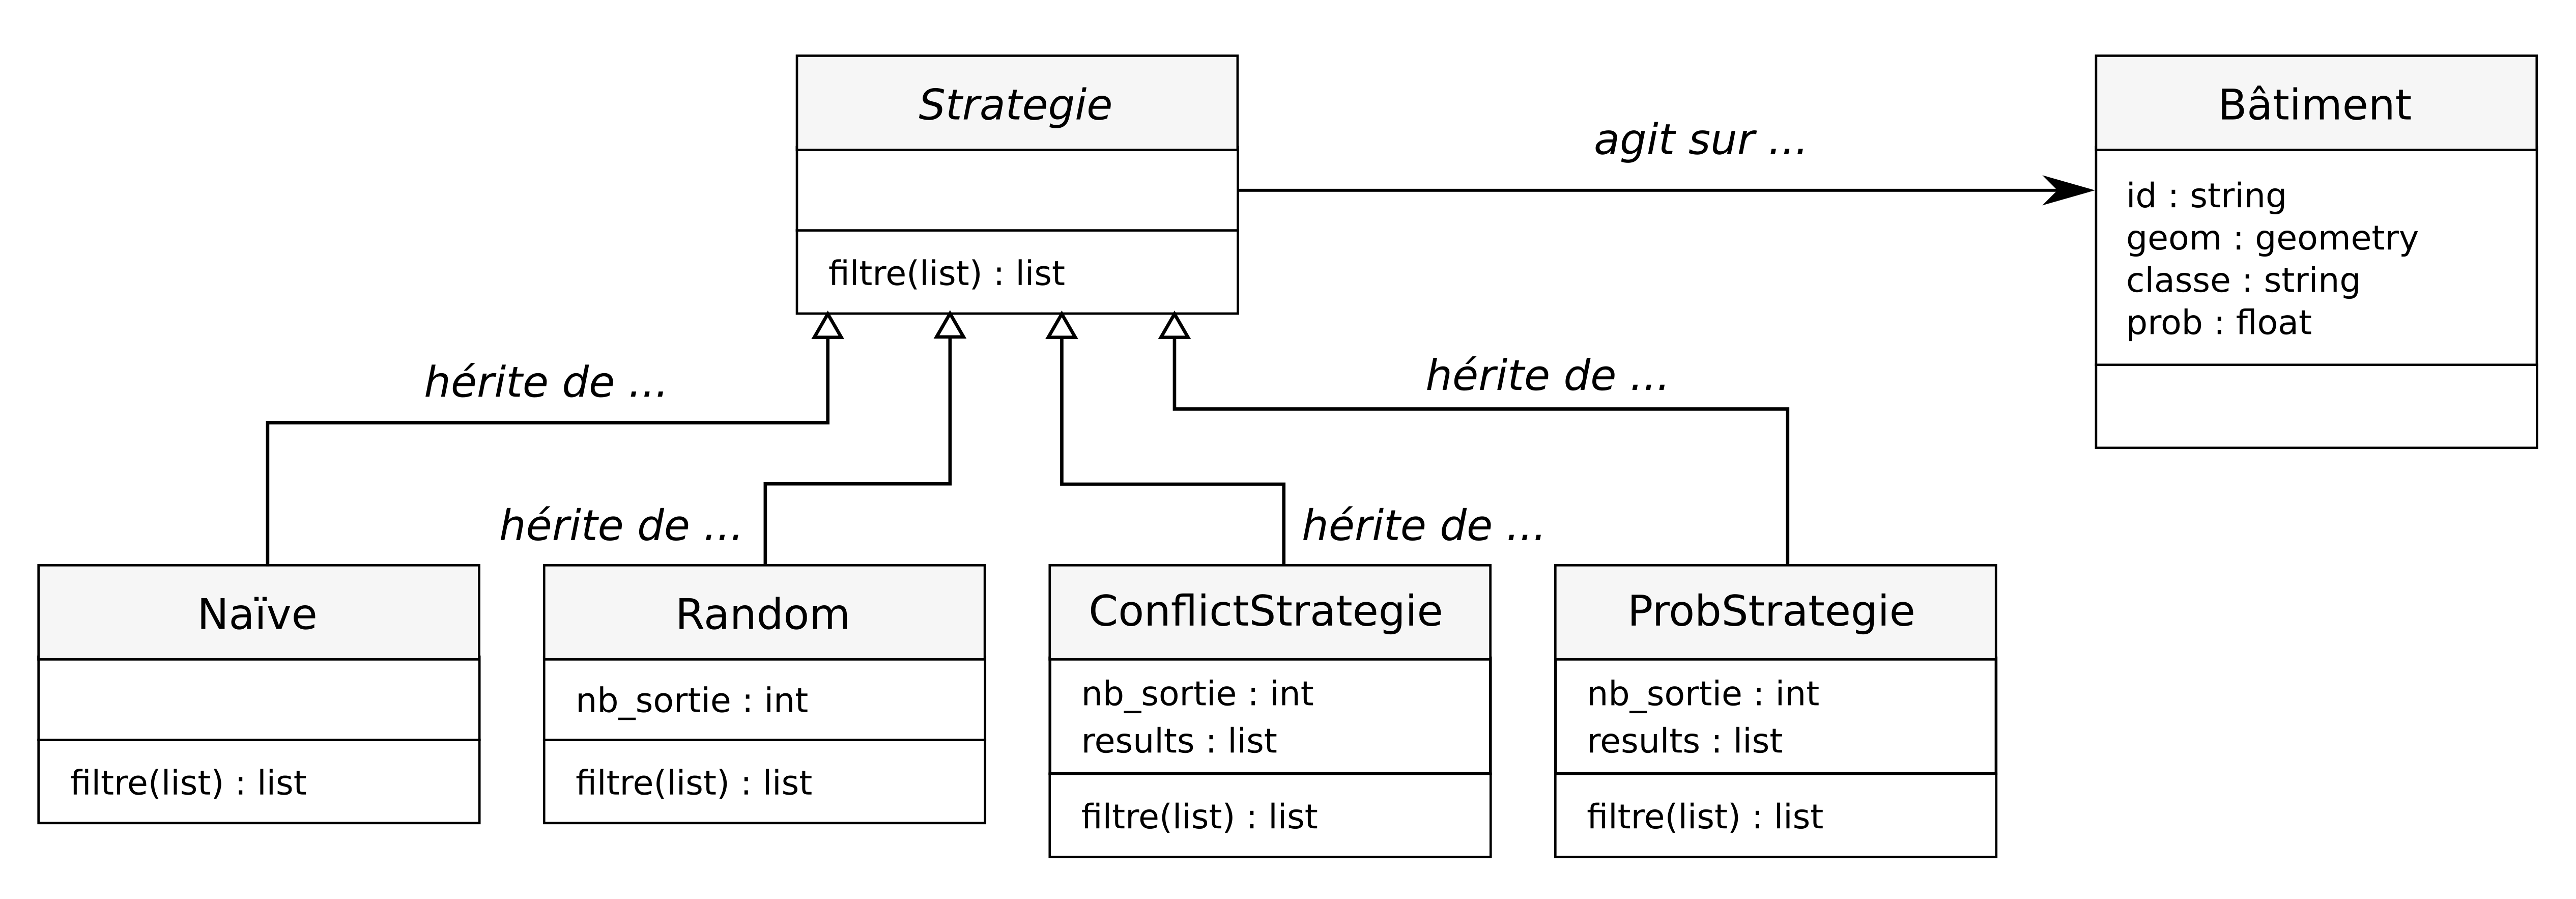
\includegraphics[scale=0.39]{diagramme_classes.png}  \\
		\caption[Diagramme de classe]{Diagramme de classe}
		\label{fig:classe}
	\end{center}
\end{figure}

\section{Maquette du projet}

Après avoir défini l'ensemble des contraintes, des données, des fonctionnalités et de leur implémentation, on réalise une première ébauche de l'interface. La fenêtre principale permet de visualiser les entités et leur classe. On prévoit aussi une fenêtre pour charger les données, et une autre pour choisir la nouvelle classe en cas de mauvaise qualification de l'erreur.

\begin{figure}[H]
	\begin{center}
		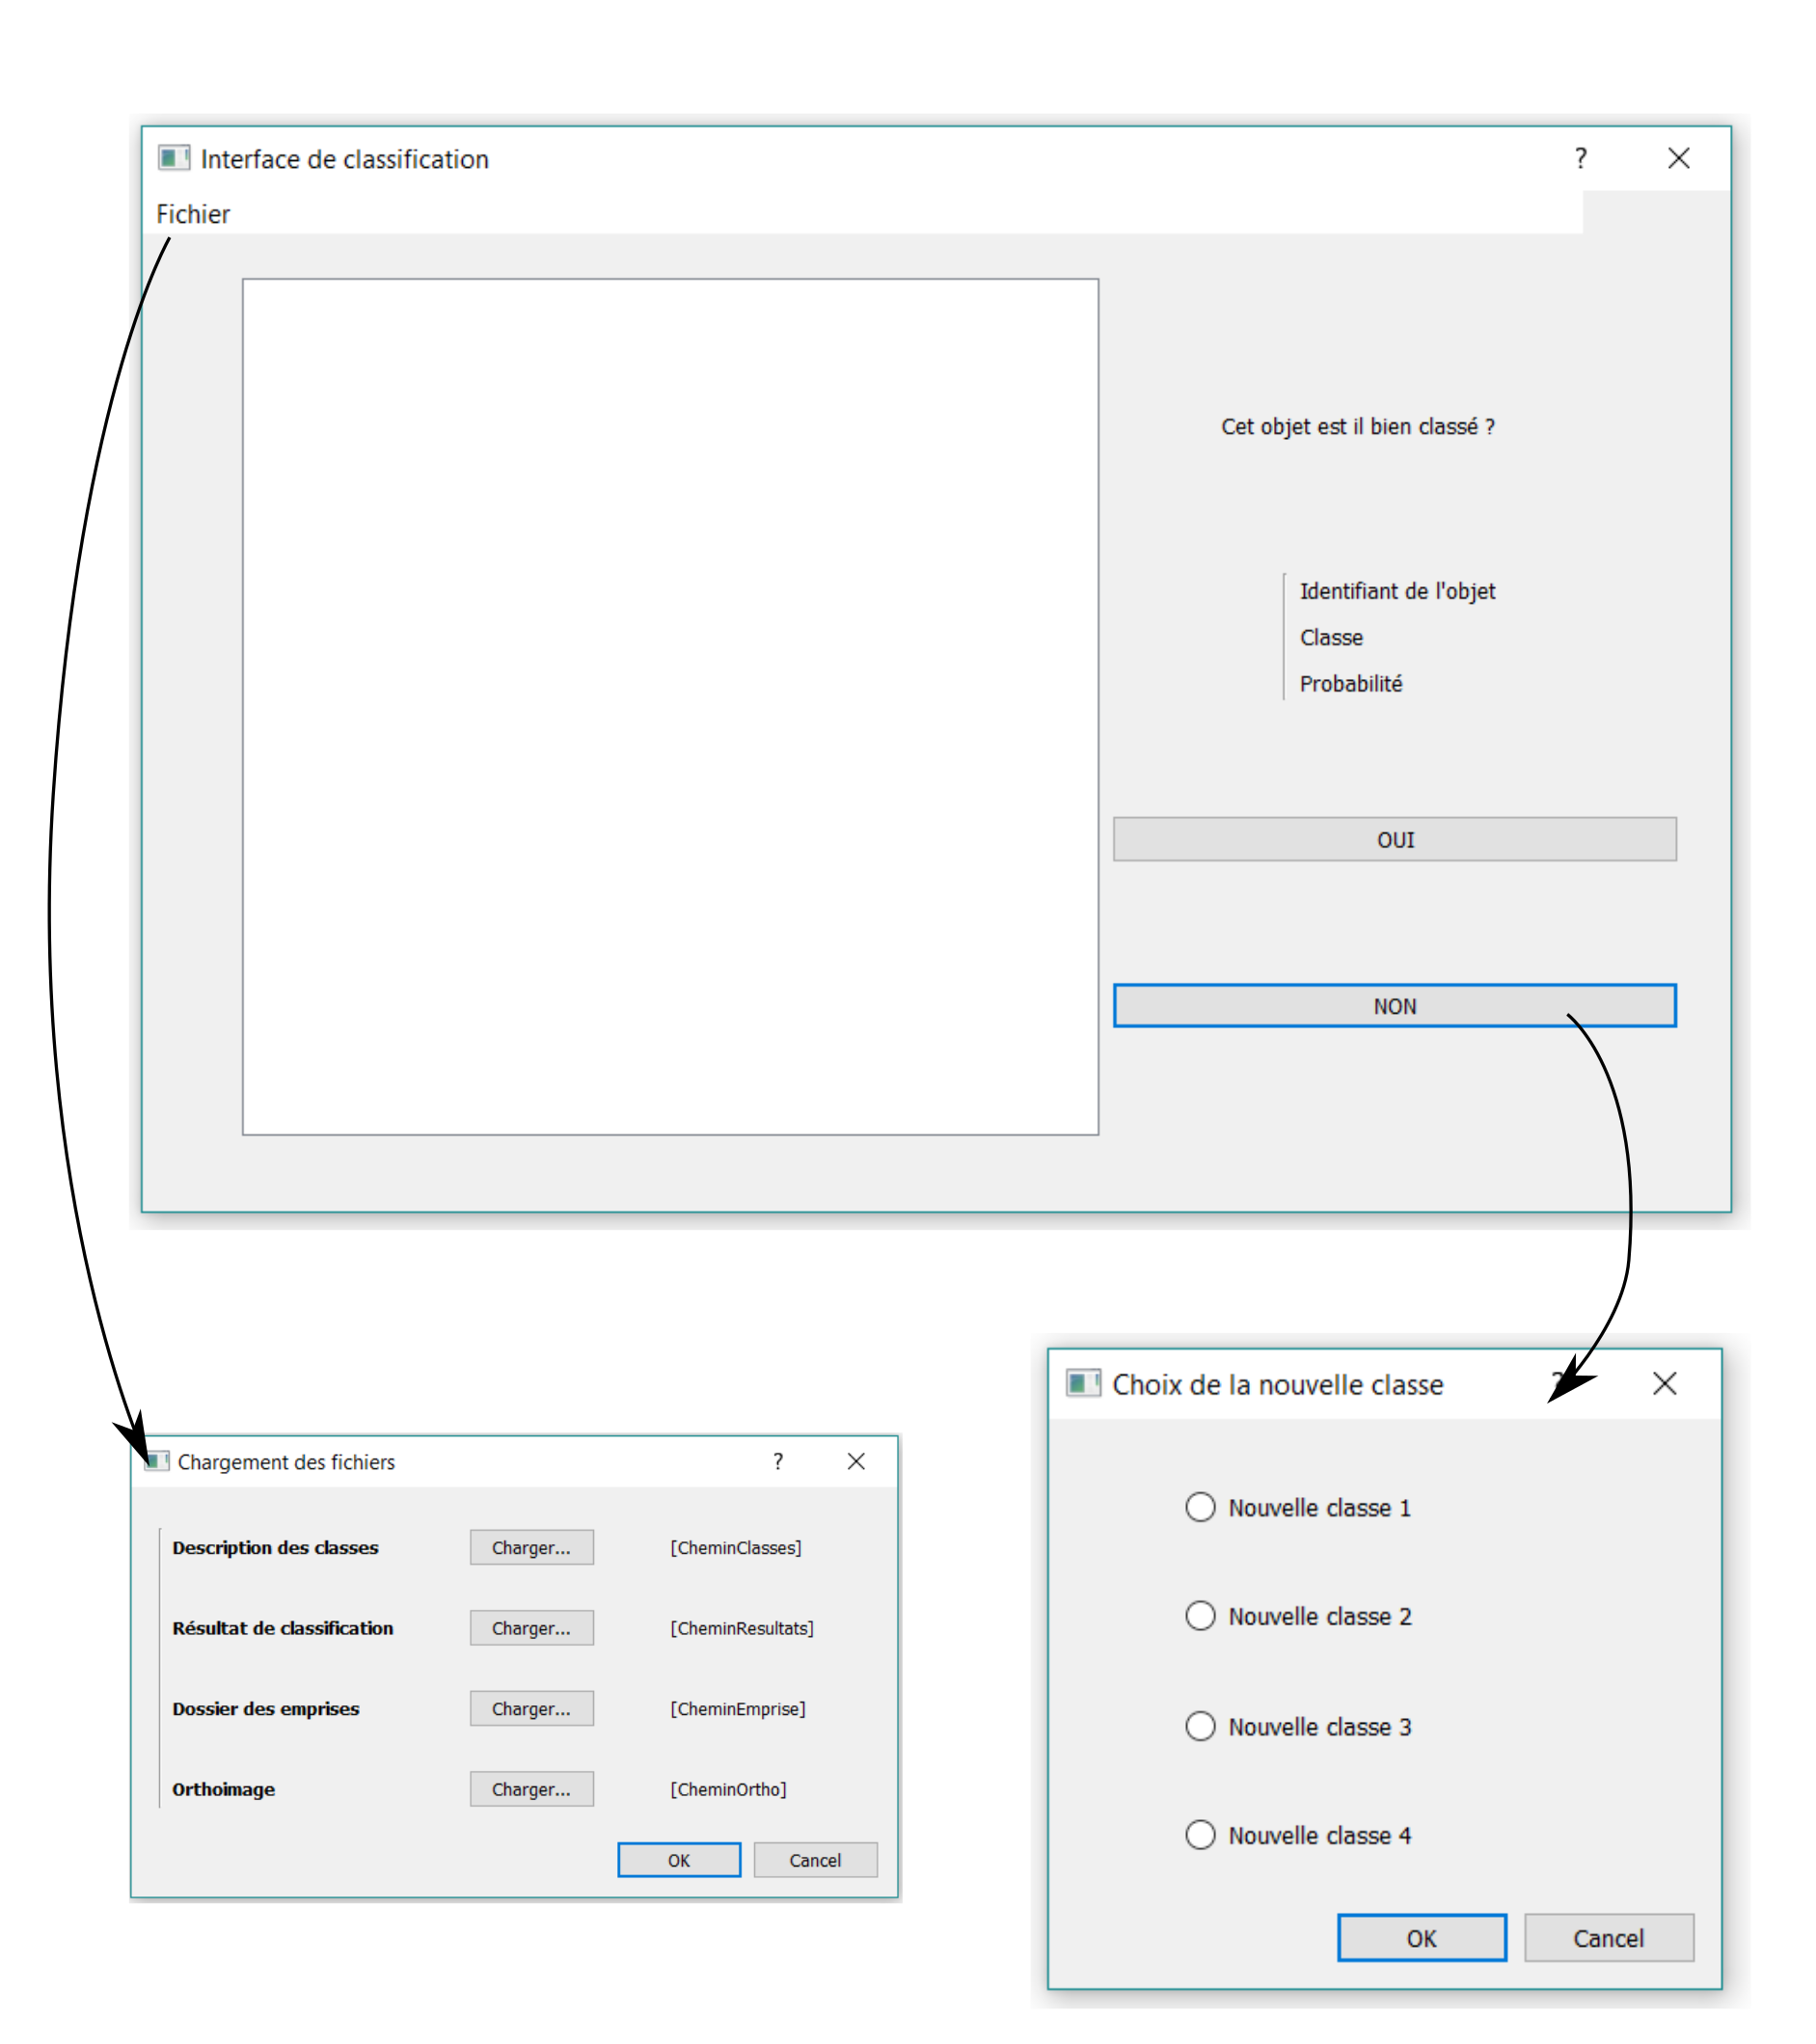
\includegraphics[scale=0.9]{Maquette.png}  \\
		\caption[Maquette de l'interface]{Maquette de l'interface.}
		\label{fig:maquette}
	\end{center}
\end{figure}

Les donnée et les fonctionnalités présentées dans ce chapitre s'appuient sur des choix techniques. Le prochain développement permettra de justifier ces choix.



